%#BIBTEX pbibtex document
%
% 計測自動制御学会システム・インテグレーション部門学術講演会2012原稿サンプルファイル
%                                           October 4, 2012
% Based on 計測自動制御学会システム・情報部門学術講演会2012原稿サンプルファイル
%                                           April 28, 2012
% Based on 第7回計測自動制御学会制御部門大会原稿サンプルファイル
%                                           October 18, 2007
% Based on 第5回計測自動制御学会制御部門大会原稿サンプルファイル
%            近野敦 konno@space.mech.tohoku.ac.jp    March 05, 2005
%
% Based on Github : yoneken/SI2012_sampleTeX
% https://github.com/yoneken/SI2012_sampleTeX
% https://github.com/yoneken/si2012.sty

\documentclass[10pt,a4paper]{jarticle}
\usepackage{style/si2015}

\usepackage{url}
\usepackage[dvips]{graphicx}
\usepackage[numbers,super,square]{natbib}
\usepackage{mathpazo}
\usepackage{color}
\usepackage{graphicx}
\usepackage{listings}
\usepackage{amsmath,amssymb}
\usepackage{bm}
\usepackage[subrefformat=parens]{subcaption}
% \makeatletter
% \def\thefigure{\thesection.\arabic{figure}}
% \@addtoreset{figure}{section}
% \makeatother

\begin{document}
\title{九州工業大学\\CIR-KIT B による独立二輪駆動型自律ロボットの開発と\\つくばチャレンジへの取り組み}
\author{○田中 良道 有田 裕太 森田 賢 西田 健(九州工業大学)}
\engauthor{
  ○Ryodo Tanaka, Yuta Arita,\\
  Masaru Morita, and Takeshi Nishida \\(Kyushu Institute of Technology)
}
\pagestyle{empty}
\maketitle\thispagestyle{empty}

\section{はじめに}
CIR-KITは,九州工業大学工学部の学部生を中心としたロボット開発チームであり,屋内外の移動を行う案内ロボット・福祉ロボットの開発に取り組んでいる.このようなロボットには,案内,荷物または搭乗者の運搬,周辺環境認識などの機能が必要である.我々はこれまでに市販の電動カートを改造したロボットを用いてこれらの課題に取り組んできたが,このロボットは前輪操舵後輪駆動型であるため小回りがきかず,屋内の走行に適さないという問題があった.そこで屋内外で活動可能な案内ロボットを目指し,小回りのきく独立二輪駆動型ロボット(KIT-C4)の開発を2014年度より続けてきた.本稿では,開発したロボットとつくばチャレンジ2016での取り組みについて報告する.

\section{ロボットの構成}
KIT-C4の外観をFig.\ref{fig:kitc4}に示す.本節では,ハードウェア構成,ソフトウェア構成について説明する.また,実際に使用したシステム全体の概要図をFig.\ref{fig:system}に示す.
\begin{figure}[tbp]
\centering
 \includegraphics[width=8cm]{fig/kitc4.eps}
 \caption{KIT-C4外観}
 \label{fig:kitc4}
\end{figure}

\begin{figure*}[tbp]
\centering
 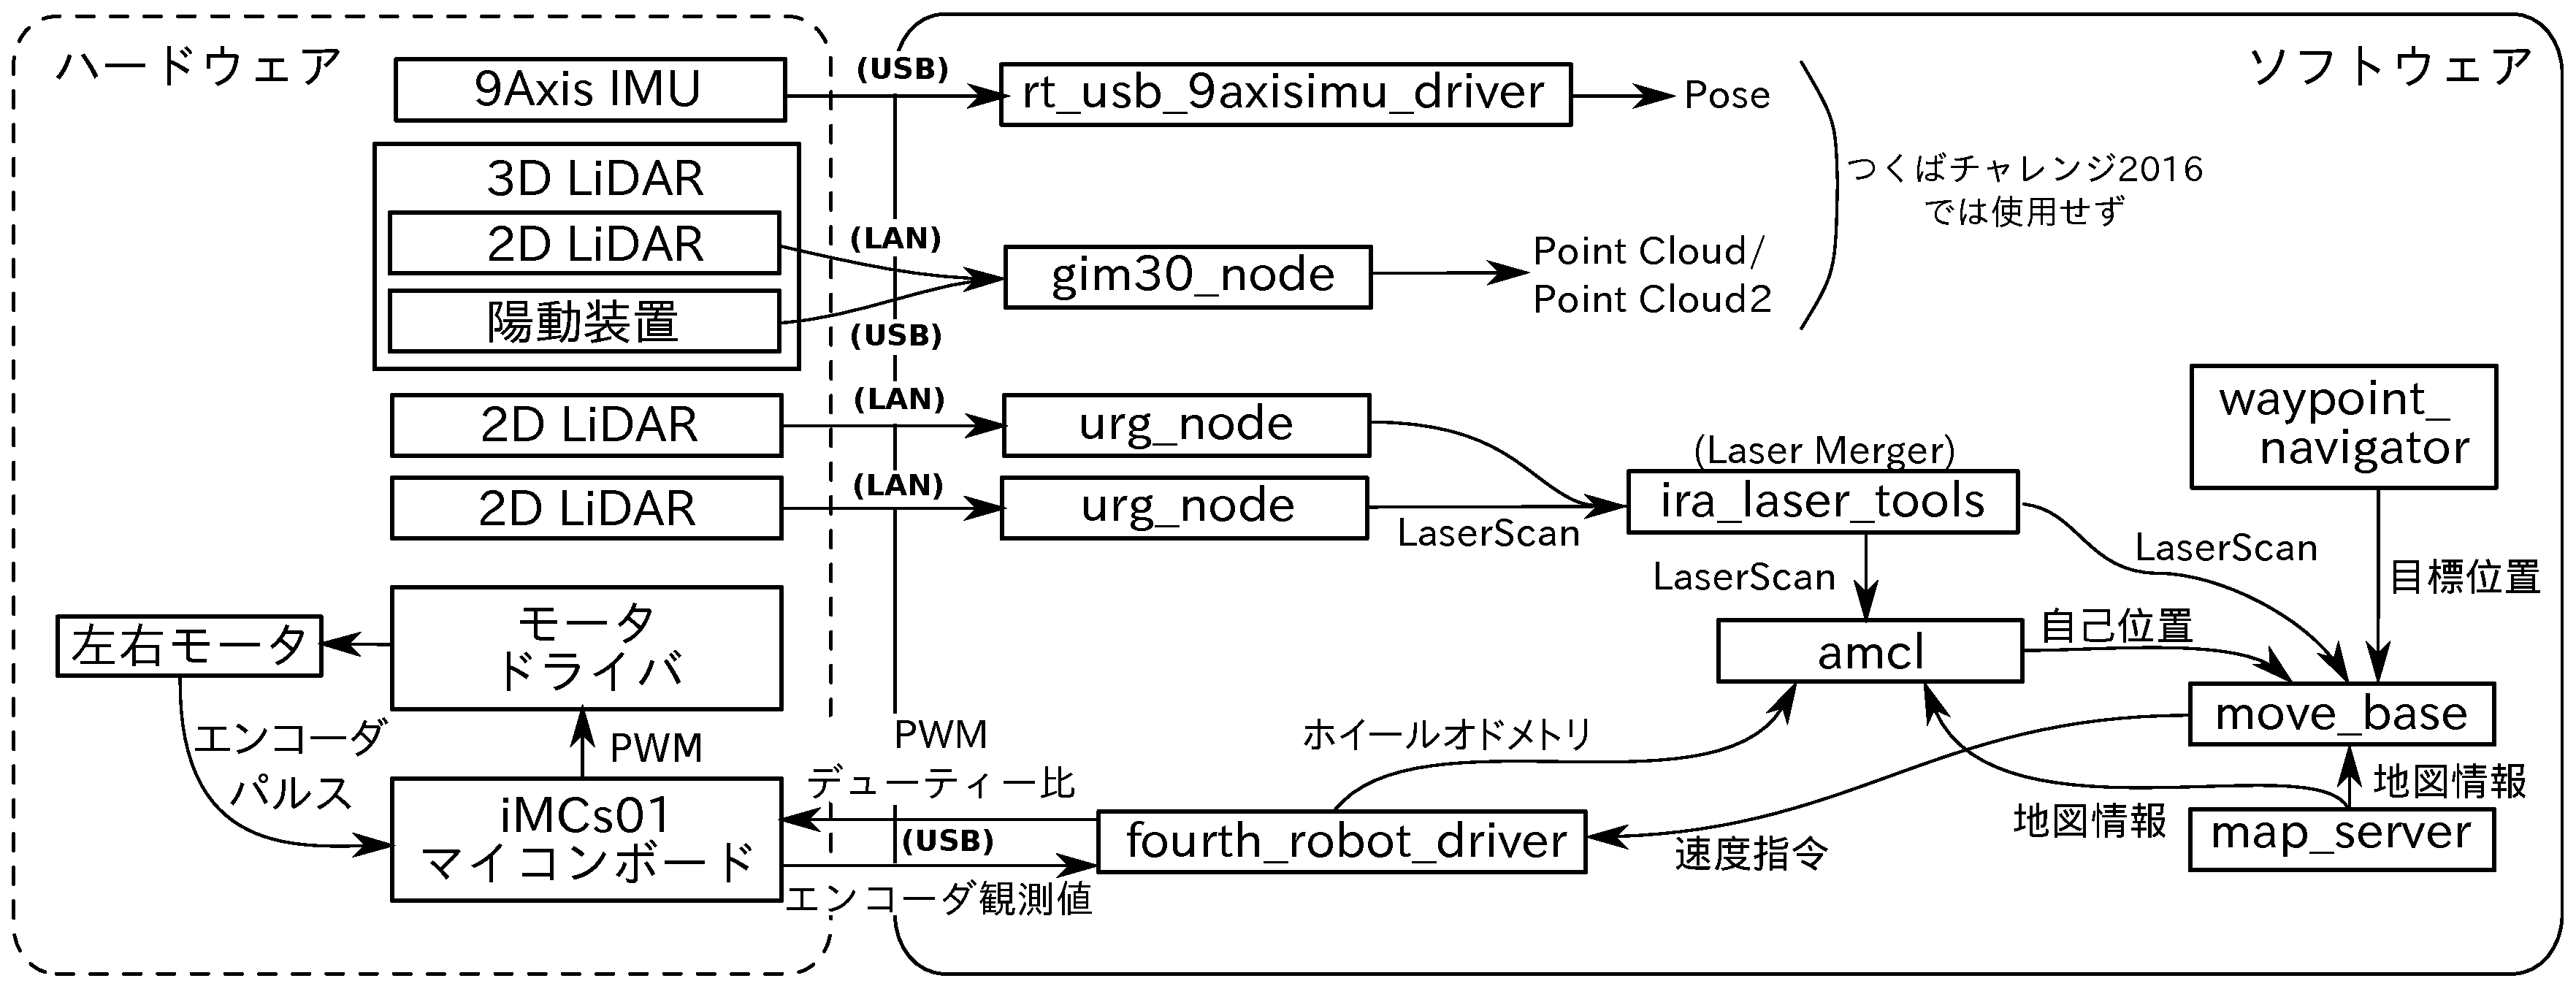
\includegraphics[width=17cm]{fig/whole_system.eps}
 \caption{システム概要}
 \label{fig:system}
\end{figure*}

\subsection{ハードウェア構成}
ハードウェア構成について,機構・駆動,センサ,制御系に分けて説明する.
\subsubsection{機構・駆動}
前述の通り,KIT-C4は独立二輪型ロボットである.16インチの自転車用のタイヤ\footnote{STRIDA:ST-WS-003}を駆動輪としており,従輪には6インチの自在キャスタ\footnote{シシク:AIJ-6-2G}を1つ用いている.駆動には,ブラシレスモータ\footnote{オリエンタルモータ:BLH5100K-30}を用いており,タイミングベルトにより駆動輪へモータの回転力を伝達している.また,モータやセンサの電源として電動自転車用のバッテリ\footnote{Panasonic:NKY452B02B}を用いており,ラップトップPCの電源には大容量モバイルバッテリ\footnote{イケショップ:BATY13818BK}を用いた.つまり,駆動・センサ系の電源とラップトップPC用の電源は別電源としており,センサ系の電源には非接触型のDC/DC変換器\footnote{Recom:REC15-2412SG}を用いることで,モータの駆動ノイズを遮断している.
\subsubsection{センサ}
環境認識のために前方・後方にそれぞれ2D LiDAR\footnote{北陽電機:UTM-30LX-EW}を,前方に3D LiDAR\footnote{移動ロボット研究所:Gim30°}を搭載している.また,ホイールオドメトリを観測するために,駆動輪の回転をタイミングベルトを介してロータリーエンコーダ\footnote{オムロン:E6B2-CWZ6C}で観測している.この他にも9軸IMUセンサ\footnote{RT Corporation:USB出力9軸IMUセンサモジュール}やDGPS\footnote{Hemisphere:A100}を搭載している.しかし,これらセンサのうちつくばチャレンジ2016で使用したのは前後の2D LiDAR,ロータリーエンコーダのみである.なお,前後の2D LiDARは観測データを統合することでロボットの周囲360[deg]を観測できるようにした.\\
 搭載したセンサの中に3DLiDARがあるが,このセンサは2D LiDARを揺動機構に載せ,振ることで3D LiDARとして機能する\cite{gim30}.これにより,Fig.\ref{fig:gim30}のような3次元情報を観測することができる.なお,揺動機構部分は1[s]周期で回転しており,Fig.\ref{fig:gim30}に示すのは,30周期分観測したときの点群情報である.

\begin{figure}[tbp]
\centering
 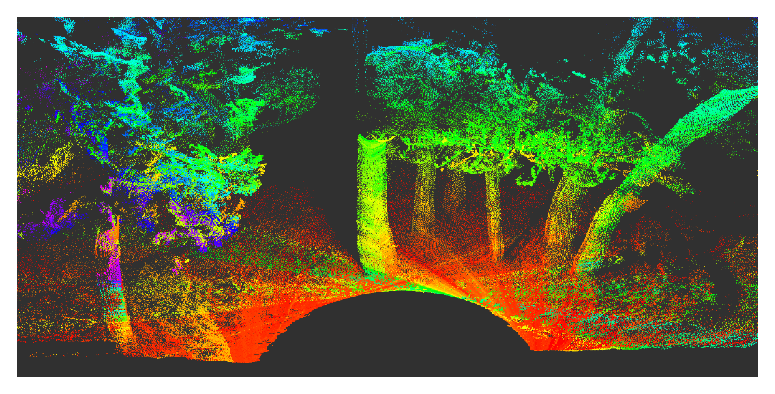
\includegraphics[width=8cm]{fig/scan.eps}
 \caption{Gim30°によるスキャンの様子}
 \label{fig:gim30}
\end{figure}

\subsubsection{制御系}
駆動モータはブラシレスモータであり,その制御にはモータ付属の専用コントローラ\footnote{オリエンタルモータ:BLHD100K}を用いている.このコントローラは,目標回転速度をPWM信号により指令することができる.開発したロボットでは,急停止・急発進を抑制するため,上位にI-Pコントローラをカスケード結合している.ここで,I-Pコントローラの観測値は,ロータリーエンコーダの観測値としている.また,ブラシレスモータの専用コントローラへのPWM入力,エンコーダ値の観測にはマイコンiMCs01\footnote{iXs Resarch:iMC01}を用いた.

\subsection{ソフトウェア構成}
\subsubsection{ROS}
ロボットのシステム統合にはROS\cite{ros}を用いている.ROSにはいくつかの特徴がある\cite{ros_okada}が,開発したロボットではソフトウェアの再利用性とROSの提供するエコシステムを特に意識した.実際,これから述べる走行手法などは同チームで開発したKIT-C3やKIT-C5と同様であり,再利用することが可能であった.これにより開発時間の短縮を図ることができた.
\subsubsection{走行手法}
自律走行には,ROSのnavigationパッケージを利用した.予め静的環境地図を製作し,地図上にWaipointを設定した後,これを辿ることで自立走行を行った.Waypointの設定には,Rviz上にIntaractive Markerを用いて設置できるソフトウェアをチームで開発し用いた.経路探索・障害物回避にはmove\_baseパッケージを,自己位置推定にはAMCLパッケージを用いた.Fig.\ref{fig:system}に示すように,AMCLでは,前後に設置した2D LiDARとホイールオドメトリ,地図情報を元に自己位置推定を行っている.前述のとおり前後に設置した2D LiDARの情報を統合しているが,ロボットの周囲360[deg]の情報を使用すると自己位置が収束しやすいだけでなく,静的地図も比較的正確に製作できることがつくばチャレンジ2015での取り組みで判明していたため,このような手法を用いた.\\
 move\_baseパッケージにおけるパスプランニングについて,グローバルパスプランニングにはNavfnの標準プランナを,ローカルパスプランニングにはDWAプランナを使用した.本走行でもこれを利用したが,利用したNavfn標準グローバルプランナは探索対象である地図の規模が大きくなるほど探索時間が長くなり,グローバルパスを計算している途中でロボットが追従できなくなるほどパスから離れてしまう現象が発生したため,本走行の走行結果は期待したよりも短くなってしまった.これについての考察は第\ref{sec:consider}節にて行う.
\subsubsection{環境地図}
環境地図の製作にはgmappingパッケージを利用した.前述の通り,レーザーセンサの情報には前後の2d LiDARの統合情報を用いた.大清水公園のみの地図には100[mm]四方の占有格子地図を,大清水公園と公園外の地図には50[mm]四方の占有格子地図を用いた.大清水公園のみの地図程度の規模であれば,Navfnの標準グローバルプランナの計算時間は走行に十分なほど高速であったが,大清水公園以外のコースを含めた地図の規模になると,前述の通り計算速度は走行に十分とは言えないほど低下した.なお大清水公園以外を含めた地図とは,つくばチャレンジ2016の課題コース全体の地図のことを指す.なお,gmappingを用いて地図を製作したのみでは,地図上に移動物体の影などが残るため,グローバルプランニング時に存在しない障害物を避けるために計算時間が増大する問題が発生する.この問題に対しては地図を製作後,画像編集ソフトを用いて人の手により修正することで対処した.

\section{物理シミュレータの活用}
開発したロボットでは,開発の効率化,実験の効率化を図るためにROS標準の物理シミュレータであるGazebo\cite{gazebo}を活用した.特にKIT-C4においては,navigationパッケージの動作実験を主な目的として使用した.結果として,ハードウェア開発とソフトウェアの開発を独立して行うことができた.また,理想の挙動を示すロボットモデルと実機を比較することで,低レイヤーの制御部分のデバッグやハードウェアの修正を効率的に行うことができた.Fig.\ref{fig:gazebo}に,開発したシミュレータの様子を示す.また,シミュレーションモデルの構築手法はインターネット上の情報共有サイトに公開している\footnote{http://qiita.com/RyodoTanaka/items/c3014fd6d0f06d12814f}.
\begin{figure}[tbh]
  \begin{minipage}[b]{1.0\linewidth}
  \centering
  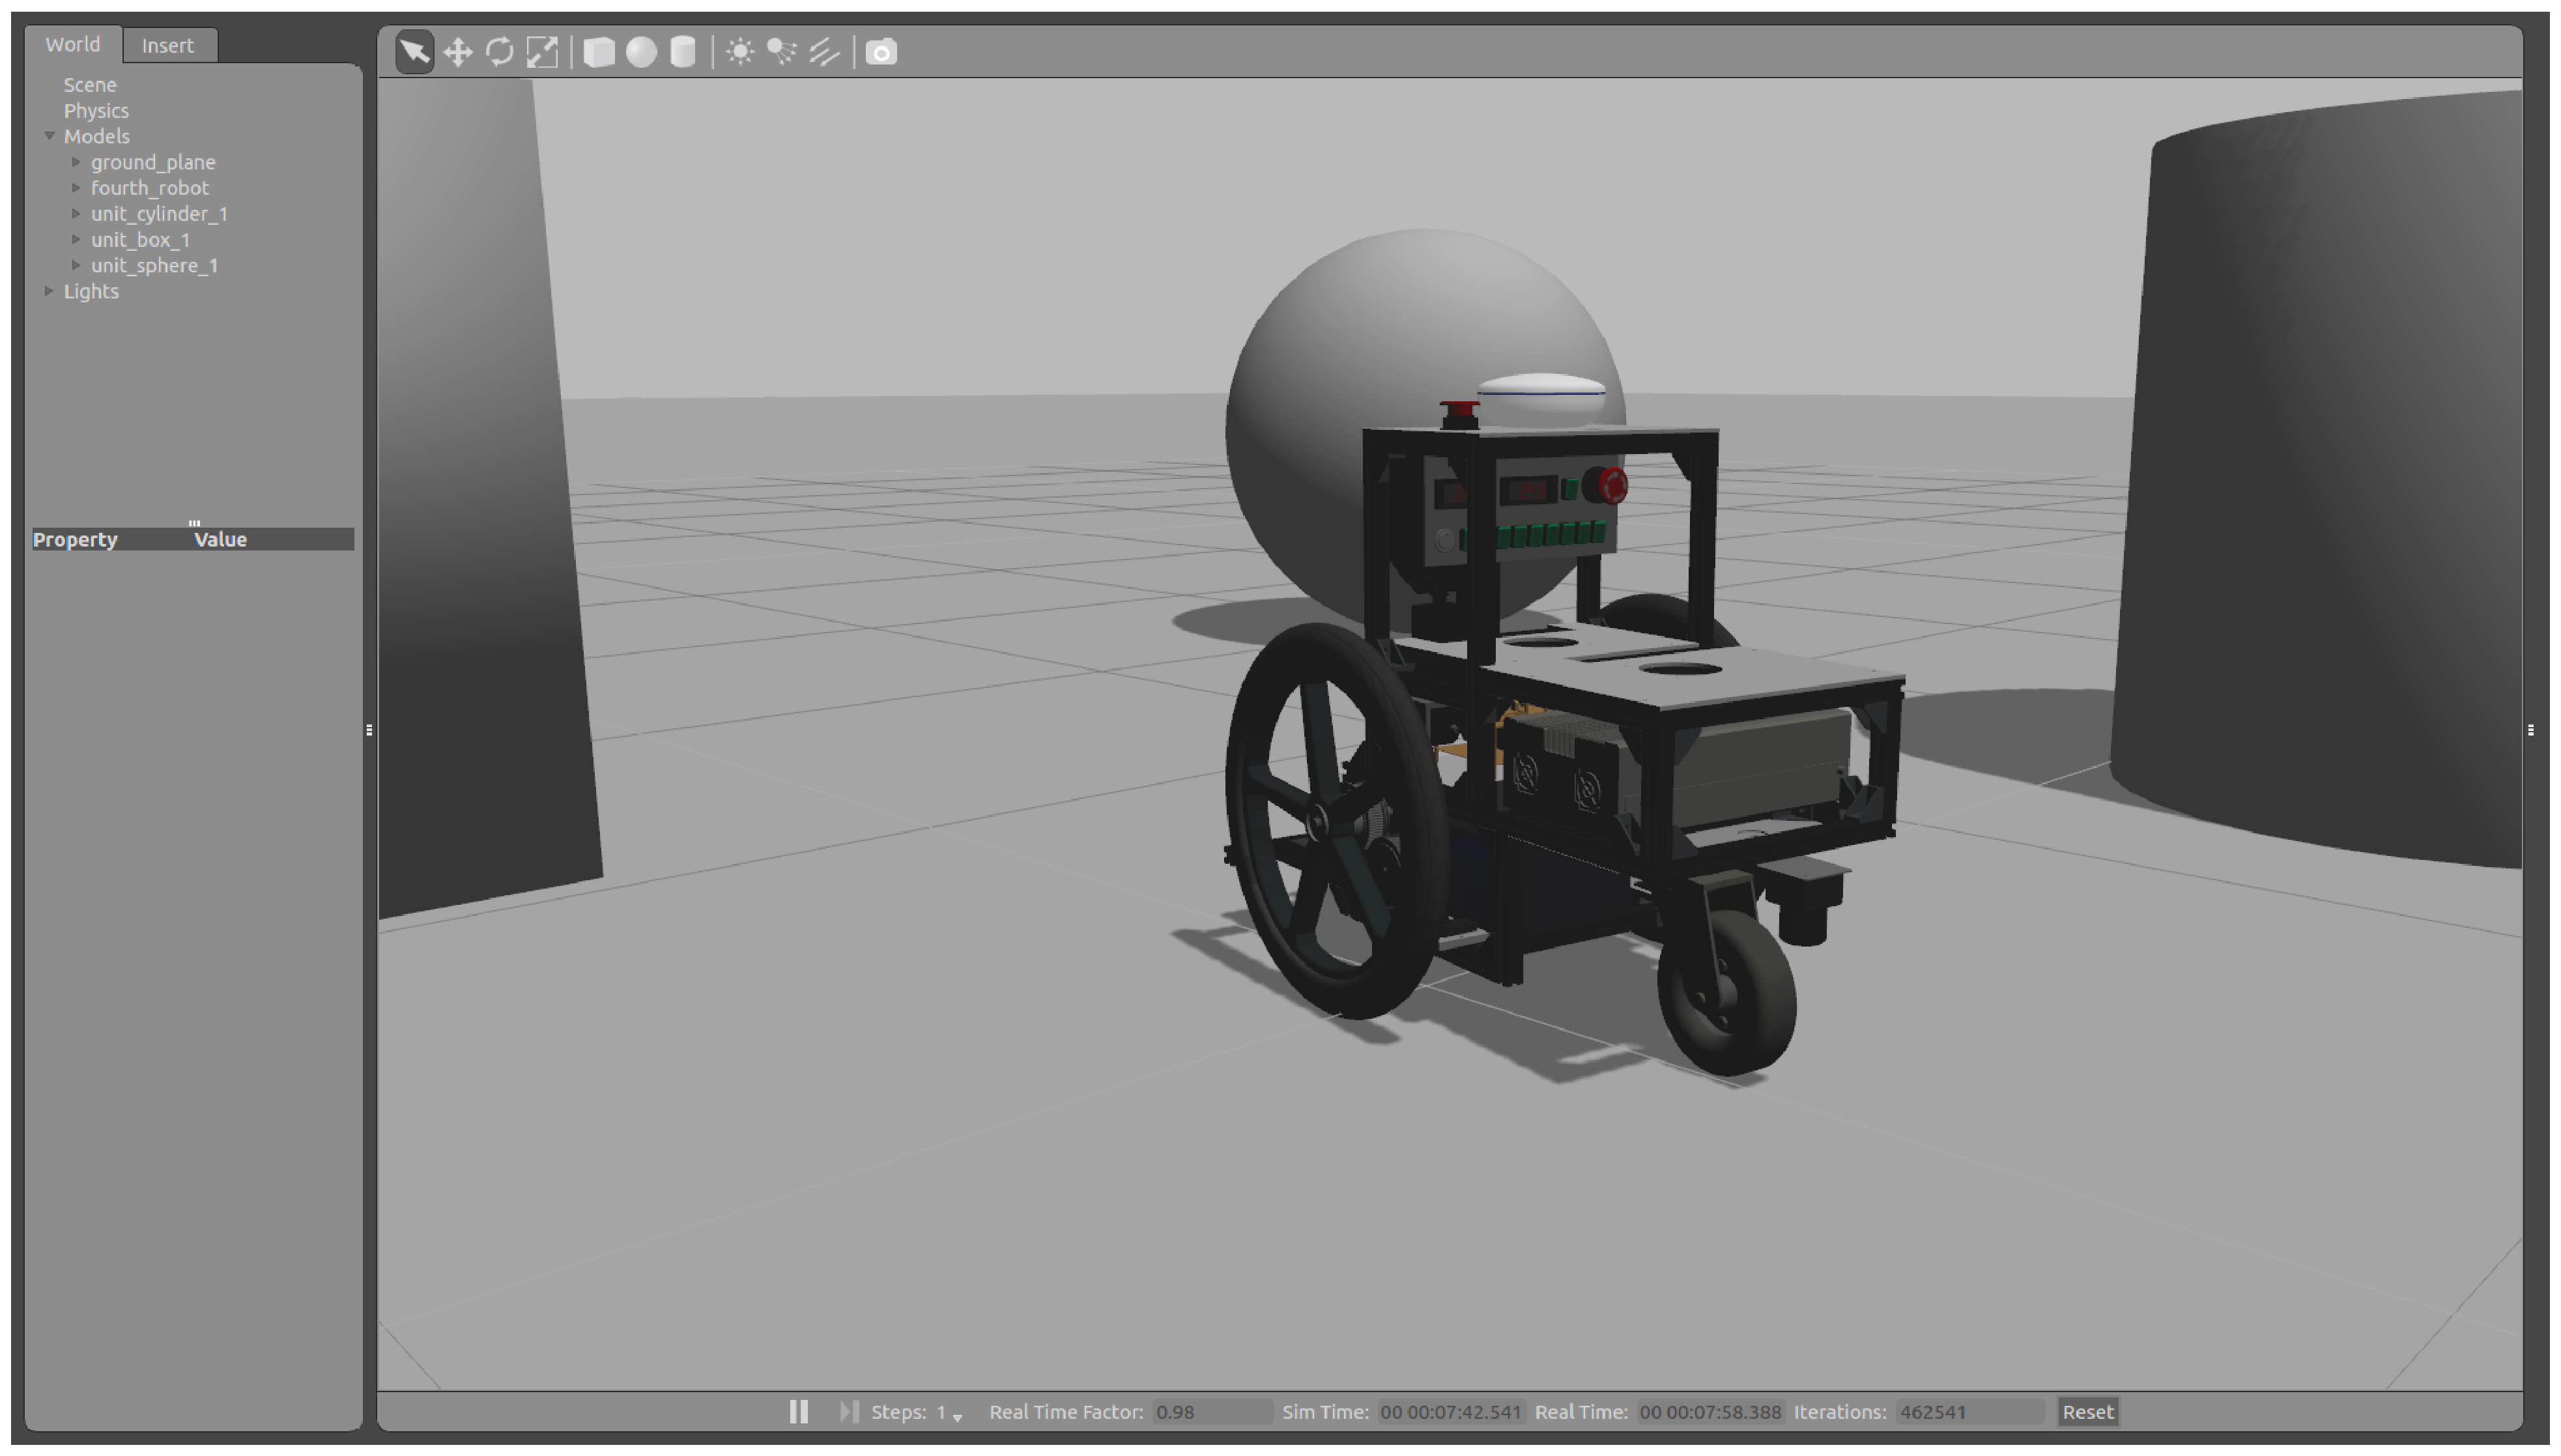
\includegraphics[keepaspectratio, width=8cm]
  {fig/gazebo.eps}
  \subcaption{Gazeboモデル}
  \end{minipage}\\
 \begin{minipage}[b]{1.0\linewidth}
  \centering
  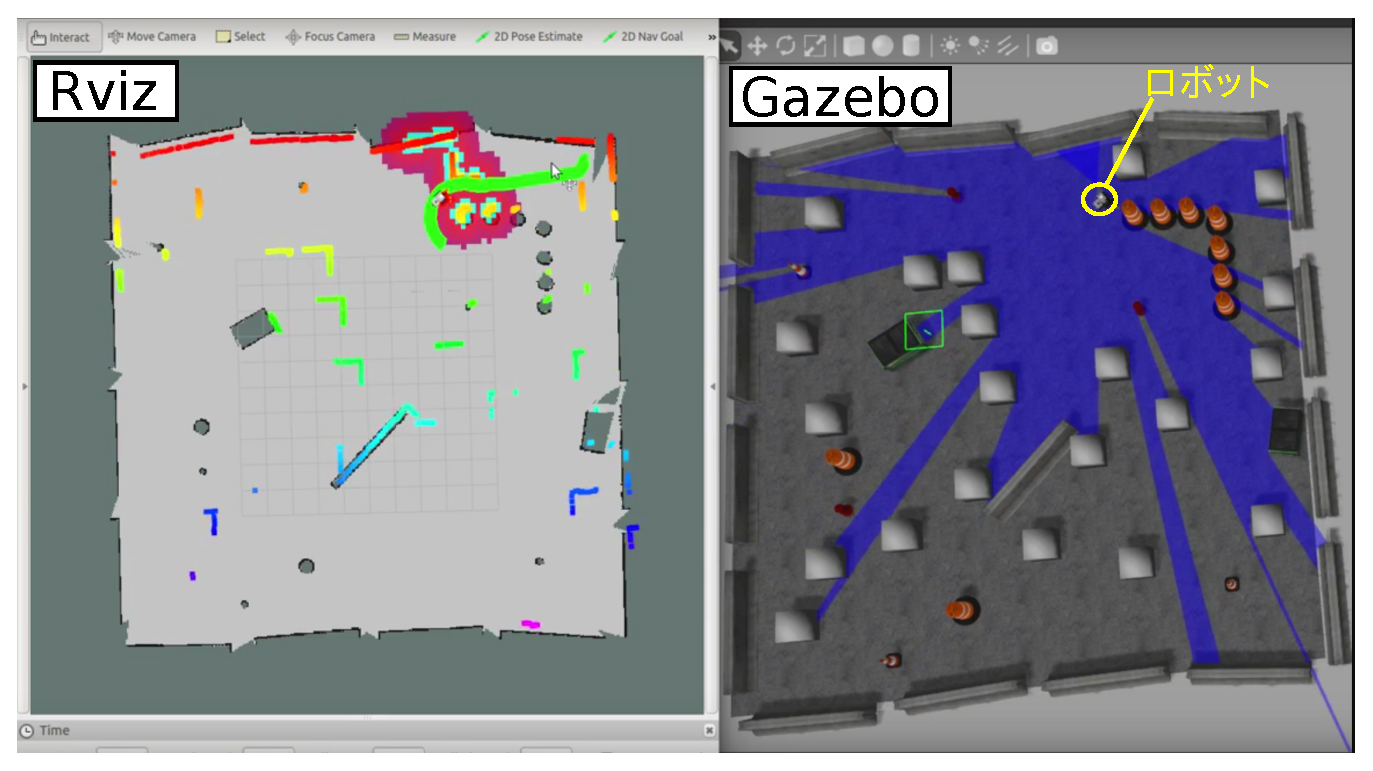
\includegraphics[keepaspectratio, width=8cm]
  {fig/navigation.eps}
  \subcaption{navigationパッケージのテストの様子}
 \end{minipage}
 \caption{製作したGazeboシミュレータ}\label{fig:gazebo}
\end{figure}
\subsection{ros\_controlについて}
Gazebo上で任意のモデルを動かすためにはros\_controlを介する必要がある.ros\_controlとは,実機とシミュレータ間で共通のコントローラを利用できるようにすることを目的としたフレームワークである.コントローラを共通化することで,アプリケーションの開発をハードウェアとソフトウェアに分かれて行い易くする効果がある.KIT-C4のシミュレーションでは,ros\_controllersに標準で提供されているdiff\_drive\_controllerを使用したが,実機のコントローラについて,つくばチャレンジ2016本走行時ではros\_controlは使用せず,以前より開発していたドライバパッケージを用いて駆動した.このドライバパッケージとは,Fig.\ref{fig:system}上のfourth\_robot\_driverを指す.

\section{つくばチャレンジ2016の結果と考察}
\label{sec:consider}
\subsection{実験走行}
静的地図の製作以前に,ハードウェアの調整に時間を有した.これは,今年から追加されたルールへの対応が主であったが,現地で指摘されなければわからない部分でもあるので,遠方から参加する我々にとっては必要不可欠な時間であったと言える.その後の静的地図製作は特に問題もなく行うことができた.しかし,確認走行時点になり,モータの異常回転によるロボットの暴走が不定期かつ頻繁に発生し,このデバッグに時間を要した.原因は,ロボットの速度算出の際にゼロ割が起こり,NaNが発生することであった.原因究明が遅れた理由として,計算過程の値をデバッグ用に記録しておらず,逐次的にプログラムを書き換える必要があった点と,ゼロ割が不定期に発生していたことが挙げられる.この点は,実験走行以前に九州工業大学内の走行実験を繰り返すことで発見・対処出来た問題と考えられるため,実験不足が露呈する結果となってしまった.一方,ゼロ割の修復後は安定して走行し,確認走行区間は到着より2日目に走破することができた.確認走行区間外の走行に関しては,実験走行に参加出来たのが2日間のみであったため,地図の製作と数回の実験のみしか行うことができなかった.そのため,大規模地図に対する最適なグローバルプランナを決定する実験を十分に行うことができず,本走行の結果へと繋がった.
\subsection{本走行}
本走行の記録は,スタート直後約30[m]地点でのリタイアとなった.コース脇の段差に従輪がスタックし,ホイールオドメトリが大幅にずれたことに起因する自己位置推定の破綻が原因である.そもそも,コース脇の段差にてスタックしてしまった理由は,課題コース全体の地図に対して,グローバルプランナの計算速度が走行に十分でないほど遅かったためである.グローバルプランニングはNavfnの標準プランナである,Global Dynamic Window Approach を用いた.このアルゴリズムでは,地図の規模が小さければ比較的高速に演算を行うことができるが,規模が大きくなると計算時間が増大する欠点がある\cite{navfn}.対処法として,関心領域のみの地図を大規模地図より切り取り,切り取った地図に対して同アルゴリズムを適用する方法が考えられる.一方で,ROSのnavigationパッケージにはこの他にもプランナが用意されており,特にcarrot\_plannerを用いる方法が最も導入コストの少ない解決法であることがチーム内の別ロボットの実験により判明した.carrot\_plannerでは,目標地点が障害物上にあった場合に障害物外に新たな目標地点を設定し直すようなプランナであるが,スタートとゴール地点は直線で結ぶのみであり探索処理を行わないため,非常に高速にグローバルパスを生成することができる.ゆえに,carrot\_plannerを用いる場合にはWaypointの間隔を短くする必要がある.

\section{開発状況}
\subsection{ハードウェア}
本年度の開発は,昨年度までに開発してきたロボットを用いたが,KIT-C4のハードウェア開発は1人で行った.これにより発生する人的リソース・開発時間の不足により,搭載したセンサをすべて活用することができない問題が起きた.一方で,人的リソースを複数台のロボット開発に分散させることで得られる知見もあった.特に,ハードウェア仕様の共通化の必要性を強く感じた.我々CIR-KITは本年度3台のロボットを開発し参加させたが,すべてのロボットの2D LiDARの取り付け位置がバラバラであった.これは,3台のロボットが静的環境地図を各々製作する必要があることを指す.取り付け位置を統一することができれば,静的環境地図を共有することができ,より開発時間を短縮することができると考えられる.
\subsection{ソフトウェア}
ハードウェア開発が1人であった一方で,上位のソフトウェア開発はROSを活用することで,他のロボットの開発成果を共有することに成功した.また,チーム全体ではGitHubを活用し,コードの共有・統合,SNS機能を利用した開発を行った.特にKIT-C4については,開発途中よりTravis CIを利用したビルドテスト環境を構築することで,ソフトウェア共有化をより行い易くすることができた.

\section{最後に}
我々の開発成果は以下のGitHub上に公開している.
\begin{description}
 \item[Gim30ドライバ]~\\ \url{https://github.com/RyodoTanaka/gim30}
 \item[KIT-C4 CAD]~\\ \url{https://github.com/CIR-KIT/4th_Robot_CAD}
 \item[KIT-C4 package]~\\ \url{https://github.com/CIR-KIT/fourth_robot_pkg}
\end{description}
今後の開発を行うにあたって参考にしていただければありがたい.

\section*{謝辞}
つくばチャレンジ実行委員会やつくば市の方々には大変貴重な実験の機会を与えて下さり,感謝いたします.
%%%%%%%%%%%%%%%%%%%%%%%%%%%%%%%%%%%%%%%%%%
\begin{thebibliography}{9}
 \bibitem{gim30} 松本光広,吉田智章,森利宏,油田信一,回転式揺動機構とSCIP-3Dコマンドシステムを用いた三次元測域センサモジュール,日本機械学会論文集,C編,75巻,760号,pp.186-195,2009.
 \bibitem{ros} Open Source Robotics Foundation,``ROS'',\url{http://www.ros.org},as of Nov 16th 2016.
 \bibitem{ros_okada} 岡田彗,ROS(ロボット・オペレーティング・システム),日本ロボット学会誌,Vol.30,No.9,pp.830-835,2012.
 \bibitem{gazebo} Open Source Robotics Foundation,``GAZEBO'',\url{http://gazebosim.org/},as of Nov 2016.
 \bibitem{navfn} Oliver Brock,Oussama Khatib,``Hith-Speed Navigation Usage the Global Dynamic Window Approach'',International Conference on Robotics \& Automation,IEEE,pp.341-346,1999.
\end{thebibliography}
%%%%%%%%%%%%%%%%%%%%%%%%%%%%%%%%%%%%%%%%%%

\end{document}
